\chapter{Theoretische Grundlagen}
Das nachfolgende Kapitel beschäftigt sich mit den theoretischen Grundlagen, die für die vorliegende Arbeit benötigt werden. Dies bezieht sich auf die Konzepte von DevOps und Continuous Delivery. Grundsätzlich kann man zwei primäre Phasen im Lebenszyklus einer Software unterscheiden. Zuerst erfolgt die Entwicklung und nachfolgend der Betrieb der Software. DevOps findet hauptsächlich in der Phase des Software-Betriebs statt und liefert Ansätze, um häufig auftretende Probleme zu bewältigen.

\section{Probleme des klassischen Software-Betriebs}
\label{sec:probleme}
Das primäre Ziel von Software ist, einen Mehrwert für die Benutzer zu schaffen. Von der initialen Idee bis zum produktiven Einsatz gibt es viele Probleme zu überwinden. Seit Ende der Neunziger werden bereits viele Probleme in der Software-Entwicklung, durch den Einsatz von agilen Entwicklungsmethoden, bewältigt. Die Probleme im Bereich des Software-Betriebs wurden dabei aber nicht berücksichtigt. Wie in der Einleitung erwähnt, versucht DevOps diese bekannten Probleme des klassischen Software-Betriebs zu lösen. Aus diesem Grund wird DevOps auch als agiler Software-Betrieb bezeichnet \cite{humble2010, peschlow2012}. In den nachfolgenden Abschnitten wird eine Auswahl bekannter Probleme aus \cite{humble2010} angeführt und durch DevOps ermöglichte Lösungen aufgezeigt.

\subsection{Manuelles Deployment einer Software}
\label{sec:problem:manuellesdeployment}
Sofware-Systeme haben meist einen hohen Grad an Komplexität. Bei den meisten Systemen ist es nahezu ausgeschlossen, dass eine einzige Person alle Komponenten überblicken und verstehen kann. Trotzdem führen viele Betriebsteams das Deployment einer neuen Software Version manuell durch. Laut \cite{humble2010} treten dabei häufig folgende Probleme auf:

Jede Tätigkeit die manuell durchgeführt wird, ist anfällig für menschliche Fehler. Sofern diese Tätigkeiten nicht sehr genau definiert und dokumentiert sind, können unterschiedliche Personen sie unterschiedlich ausführen. Wird der Prozess wiederholt, so ist nicht sichergestellt, dass er genau gleich durchgeführt wird wie zuvor. Das Ergebnis des Prozesses ist somit nicht deterministisch. Dies hat zur Folge, dass der Prozess nicht nachvollziehbar ist und somit die Analyse von Problemen erheblich erschwert wird. Jede einzelne Tätigkeit muss nachvollziehbar sein. Wenn das Problem erst einige Zeit nach der Durchführung auftritt, ist dies meist nicht mehr möglich. Im schlimmsten Fall überblicken im Unternehmen nur einzelne Personen einen gesamten Prozess. Die Durchführung ist dann immer von diesen Personen abhängig.

Ein weiteres Problem des manuellen Deployments ist, die dafür benötigte Zeit. Je mehr Infrastrukturkomponenten bei einem Release betroffen sind, desto aufwändiger wird das Deployment. Vor allem bei verteilten Applikationen sind meist viele Server betroffen. Je nach Art des Deployments (siehe Abschnitt \ref{sec:devops:pipeline}) ist die Applikation während dieses Vorgangs für die Benutzer nicht verfügbar. Zusätzlich zu den Kosten für die Arbeitszeit der Mitarbeiter, kommen noch Wertverluste durch Nicht-Erreichbarkeit der Applikation hinzu. Dies verursacht beispielsweise negative Reputation oder Umsatzeinbußen bei Onlineshops. Durch den nicht deterministischen Ausgang eines manuellen Deployments, ist nicht sichergestellt, dass die neue Version nach dem Deployment korrekt funktioniert.

Folglich beinhaltet manuelles Deployment ein hohes Maß an Risiko und ist fehleranfällig. Aus diesem Grund sind Releases in vielen Unternehmen eine kritische Angelegenheit, mit der oft mehrere Mitarbeiter über einen längeren Zeitraum beschäftigt sind. Deployments werden deswegen weitgehend vermieden, wodurch die Probleme aber eher verstärkt anstatt vermindern werden. DevOps und Continuous Delivery setzen deswegen auf die vollständige Automatisierung dieser Aufgaben (Abschnitt \ref{sec:automation:aufgaben}). Wenn alle Tätigkeiten automatisiert erfolgen ist sichergestellt, dass sie jedes mal in genau der gleichen Reihenfolge und gleichen Art durchgeführt werden. Der Ausgang des Prozesses ist somit deterministisch und kann jederzeit nachvollzogen werden. Außerdem sind während eines Deployments keine Mitarbeiter beschäftigt und das Deployment ist in den meisten Fällen schneller abgeschlossen. Die Kosten und Risiken reduzieren sich erheblich und die Effizienz steigt. Als Nachteil ist allerdings anzuführen, dass die Umsetzung einen großen initialen Aufwand erfordert. Auf diesen benötigten Aufwand wird in Kapitel \ref{sec:implementierung} genauer eingegangen.

\subsection{Lange Release- und Feedbackzyklen}
\label{sec:releasezyklen}
Mit agilen Entwicklungsmethoden können in der Entwicklung kurze Releasezyklen erreicht werden. Ein klassischer Betrieb kann damit aber nicht schritthalten. Hier betragen die Releasezyklen oft einige Monate, bis eine neue Software Version in Produktion deployed ist. Diese langen Zyklen haben laut \cite{humble2010} folgende Auswirkungen:

Je länger die Zyklen sind, desto größer ist das sogenannte Time-to-Market. Wird eine neue Funktion umgesetzt, so verursacht die Entwicklung dieser Funktion zuerst ausschließlich Kosten. Erst wenn die neue Funktion in der Applikation verfügbar ist, ergibt sich ein Wert für die Kunden. Je länger diese Zeit dauert, desto später wird ein Wert generiert. Im schlimmsten Fall wird zum Zeitpunkt des Deployments, die Funktion gar nicht mehr benötigt. Es sind also nur Kosten entstanden aber kein Wert. Ändern sich die Anforderungen der Kunden, kann nicht mit der nötigen Flexibilität reagiert werden. Dies führt zu unzufriedenen Kunden und im schlimmsten Fall zu deren Verlust. Des Weiteren müssen die Kunden entsprechend lange warten, bis geforderte Verbesserungen in der Applikation verfügbar sind. Dieser Nachteil betrifft vor allem die Fehlerbehebung. Wird ein Fehler erkannt, dauert es im schlimmsten Fall einen kompletten Zyklus, bis er behoben ist. Bei kritischen Fehlern ist dies oft nicht möglich und es wird ein außerplanmäßiges Deployment benötigt.

Je früher die Entwickler Feedback zu ihrer Arbeit bekommen, desto mehr sind sie noch mit dem nötigen Kontext vertraut. Fehler können so schneller gefunden und behoben werden. Erfolgt aufgrund langer Zyklen erst spät Rückmeldung, ist für die Fehlerbehebung ein Kontextwechsel notwendig. Dies bedingt meist eine längere Dauer für die Fehlerbehebung.

Gängige Praxis ist es, durch möglichst wenige Releases, das dabei auftretende Risiko beim Deployment zu vermeiden. In der Realität steigt aber das Risiko, je länger die Releasezyklen sind. Bei einem langen Zyklus sind viele Änderungen in einem Release enthalten. Die Änderungen betreffen viele Bereiche der Infrastruktur, die im Zuge des Deployments verändert werden. Treten anschließend Fehler auf, ist es schwer nachzuvollziehen, welche der Änderungen diesen Fehler verursacht. Bei kurzen Releasezyklen wäre die Menge der Änderungen hingegen überschaubar. Die Ursache für einen Fehler kann leicht festgestellt werden. Auch ein Rollback auf eine frühere Version, ist bei wenigen Änderungen meist leichter durchzuführen. Der Stressfaktor verringert sich erheblich für alle beteiligten Personen. Ist der Deploymentprozess automatisiert, kann dieser schnell und oft durchgeführt werden. Kurze Releasezyklen sind daher einfach zu erreichen und entlasten das Personal.

\subsection{Kein Konfigurationsmanagement für die Infrastruktur}
\label{sec:probleme:infrastruktur}
Der Software-Betrieb stellt für eine Applikation die benötigte Infrastruktur zur Verfügung. Die Verwaltung dieser Infrastruktur wird meist manuell durchgeführt. Die manuelle Verwaltung birgt laut \cite{humble2010} folgende vielfältige Gefahren:

Neben der produktiven Infrastruktur, müssen meist noch weitere Testumgebungen verwaltet werden. Alle Umgebungen sollten dabei den gleichen Stand an Konfiguration aufweisen. Ist dies nicht der Fall, so kann ein Deployment zwar auf der Testumgebung, nicht aber auf der produktiven Umgebung erfolgreich sein. Je weiter die Konfigurationen der einzelnen Umgebungen auseinander laufen, desto ineffizienter werden Tests. Anhand der Tests kann keine Aussage mehr getroffen werden, ob die neue Version auf der produktiven Umgebung einwandfrei funktioniert. Bei verteilten Applikationen muss sichergestellt werden, dass alle Maschinen des Clusters dieselbe Konfiguration aufweisen. Ansonsten können Unterschiede in der Konfiguration zu schwer reproduzierbaren Fehlern führen. Die Analyse und Behebung solcher Fehler erfordert demnach viel Zeit.

Wenn Umgebungen manuell verwaltet werden, ist die Menge an Umgebungen meist begrenzt. Spezielle Umgebungen für Tests von experimentellen Entwicklungen, die Änderungen an der Infrastruktur benötigen, sind dabei nicht vorgesehen.  Solche Tests müssen entweder auf einer bestehenden Umgebung durchgeführt oder es muss eine neue Umgebung aufgebaut werden. Der Aufbau einer Umgebung ist allerdings mit viel Aufwand und Kosten verbunden. Wird auf bestehenden Umgebungen getestet, so sind die Tests des herkömmlichen Releasezyklus blockiert. Es ist also schwierig, experimentelle und komplexe Änderungen ausreichend zu testen.

Ist die Verwaltung der Infrastruktur ebenfalls automatisiert, so können diese Probleme gelöst werden (siehe Abschnitt \ref{sec:devops:infrastructureascode}). Die Infrastruktur wird dadurch nachvollziehbar und reproduzierbar. Unterschiedliche Konfigurationen werden verhindert, da die Prozesse auf jeder Maschine immer gleich ausgeführt werden. Ebenso können ganze Umgebungen ohne erheblichen Aufwand aufgebaut und wieder abgerissen werden.

\subsection{Distanz zwischen Entwicklung und Betrieb}
\label{sec:problem:kluft}
Ein Problem das DevOps immer wieder anspricht, ist die Distanz zwischen Software-Entwicklung und Betrieb. Beide Abteilungen sind maßgeblich an der Bereitstellung von Applikationen für die Kunden beteiligt. Herrscht zwischen diesen Abteilungen eine schlechte Zusammenarbeit, kommt es laut \cite{peschlow2012} meist zu folgenden Problemen:

Während der Entwicklung werden vom Entwicklerteam oft Annahmen über die produktive Umgebung getroffen. Dies kann dazu führen, dass die Applikation zwar lokal auf der Entwickler-Maschine läuft, aber nach einem Deployment nicht in Produktion funktioniert. Hier kommt es oft dazu, dass sich Entwicklung und Betrieb die Schuld gegenseitig zuweisen, anstatt gemeinsam an einer Problemlösung zu arbeiten \cite{peschlow2012}. Releases sind deshalb oft sehr aufwändig und benötigen viel Zeit, da umfangreiche Kommunikation zwischen Entwicklung und Betrieb nötig ist.

Ein weiteres Problem ist, dass diese Abteilungen unterschiedliche Ziele verfolgen, die sich teilweise gegenseitig widersprechen \cite{peschlow2012, brown2014}. Ziel der Entwicklung ist es, möglichst rasch und oft Änderungen zu veröffentlichen, um die Applikation zu verbessern. Der Betrieb verfolgt das Ziel eine stabile Plattform bereitzustellen und wird meist anhand der Verfügbarkeit der Applikationen bewertet. Jede Änderung birgt dabei ein Risiko für dieses Ziel und hat eventuell eine Ausfallzeit zur Folge\footnote{Gemäß des Sprichworts \cite{brown2014}: "Never change a running system"}. Daher sollten nur ausreichend getestete Änderungen deployed werden. Dies bewirkt allerdings lange Releasezyklen und spricht gegen das Ziel der Entwicklung.

Deswegen befasst sich DevOps neben den technologischen Themen auch speziell mit der Unternehmenskultur. Es bietet Konzepte wie die Zusammenarbeit verbessert und die Kommunikation vereinfacht werden kann. Auf diese Lösungen wird in Abschnitt \ref{sec:devops:firmenkultur} genauer eingegangen.

\section{DevOps und Continuous Delivery}
DevOps nahm seinen Anfang im Jahr 2010, als Patrick Debois eine Konferenz namens DevOpsDays veranstaltete \cite{peschlow2012}. DevOps bedeutet dabei die Verschmelzung der beiden Bereiche der Entwicklung (\textbf{Dev}elopment) und des Betriebs (\textbf{Op}eration\textbf{s}) für Applikationen. Allerdings fehlte damals eine genaue Definition des Begriffes und lieferte somit viel Interpretationsspielraum. Bis 2015 hat der Begriff bereits eine genauere Bedeutung erhalten. So versteht man heutzutage unter DevOps vor allem die Automatisierung von Prozessen, um diese effizienter und resistenter gegen Fehler zu gestalten \cite{peschlow2012, brown2014}. Ebenso ist das Abbauen von Hürden und die Optimierung von Prozessen\footnote{Im Englischen oft mit \textbf{Reducing Waste} bezeichnet} ein Hauptaspekt von DevOps. Ähnliche Ansätze spiegeln sich in der aktuell aufkommenden Lean-Bewegung wieder \cite{humble2014}.

Der Begriff Continuous Delivery (CD) wurde im Jahr 2010 maßgeblich von \cite{humble2010} geprägt. Allerdings ist die Definition ebenfalls unpräzise. \cite{fowler2013} und \cite{wolff2014} versuchen dem Begriff eine genauere Bedeutung zu geben und bezeichnen Continuous Delivery als die Fähigkeit, jederzeit und ohne erheblichen Aufwand Änderungen auf Produktion ausrollen zu können. CD ist die Weiterführung von Continuous Integration (CI), wie es in der Entwicklung schon gängige Praxis ist. Die Applikation wird dabei nicht nur gebaut, sondern auch sofort getestet und ausgerollt. Jede Änderung hat ein sofortiges Deployment zur Folge und reduziert somit die Release- und Feedbackzyklen auf ein Minimum. Hierfür ist es ebenfalls notwendig, Prozesse zu automatisieren. DevOps ermöglicht also erst die Umsetzung von Continuous Delivery \cite{schroeder2015}. Das hauptsächliche Anwendungsgebiet von DevOps und Continuous Delivery ist der Web-Bereich, wo Applikationen auf Servern betrieben werden. Allerdings können viele Ansätze und Prinzipien auch auf andere Gebiete der Software-Entwicklung und des Betriebs adaptiert werden. Die vorliegende Arbeit beschränkt sich auf den genannten Hauptbereich.

\subsection{Grundprinzip}
\label{sec:grundprinzipien}
Wie man aus den gängigen Beschreibungen von \cite{peschlow2012, brown2014, wolff2014} herauslesen kann, ist das Grundprinzip von DevOps die Steigerung der Effizienz\footnote{Definition: Wirtschaftlichkeit, Maß für den eingesetzten Aufwand zur Erreichung eines Zieles} bei gleichbleibender Effektivität\footnote{Definition: Wirksamkeit, Maß für das Erreichen eines definierten Zieles}. Hürden sollen abgebaut und Prozesse optimiert werden, um einerseits die Kosten zu senken und andererseits mehr Ressourcen für die Weiterentwicklung der Plattform zur Verfügung zu haben.

\begin{figure}[ht]
	\centering
	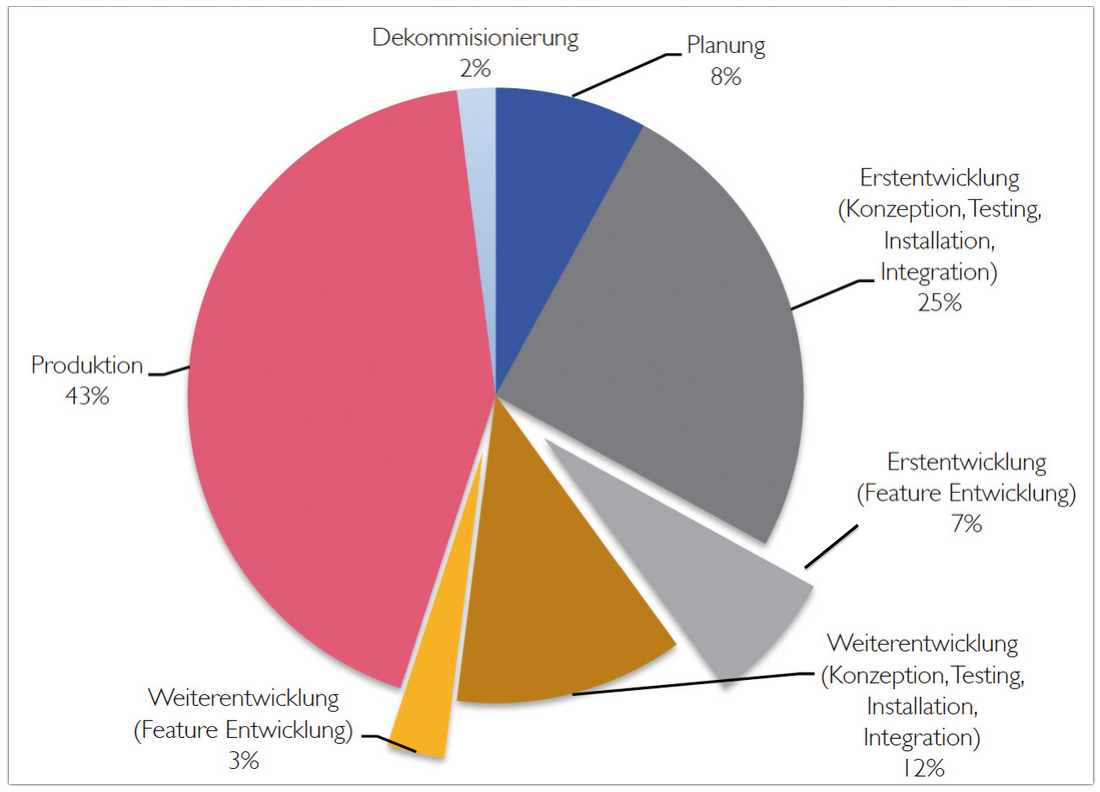
\includegraphics[width=0.9\textwidth]{img/budget_vorher.png}
	\caption[Budgetverteilung einer Applikation ohne DevOps, aus \cite{siprell2014}]{Verteilung des Budgets einer Applikation auf die unterschiedlichen Bereiche ohne DevOps, während ihres gesamten Lebenszyklus, aus \cite{siprell2014}}
	\label{fig:grundprinzip:budget_vorher}
\end{figure}  

Folgendes Beispiel führt \cite{siprell2014} an, um die Wirtschaftlichkeit von DevOps zu verdeutlichen. \autoref{fig:grundprinzip:budget_vorher} zeigt die Verteilung des Budgets einer Applikation in ihrem Lebenszyklus. Zählt man die Bereiche für Erstentwicklung (graue Bereiche) und Weiterentwicklung (orange Bereiche) zusammen, so beträgt der Anteil für die Entwicklung 47\% des Gesamtbudgets. Dabei sind allerdings Konzeption, Testen und Installation inkludiert. Betrachtet man rein den Anteil für die Entwicklung, so beträgt dieser lediglich 10\%. Durch DevOps können die Kosten vieler Bereiche reduziert werden. Auf Grund der häufigen Releases und das schnelle Feedback, muss in der Planungsphase nicht mehr jedes Szenario aufs kleinste Detail analysiert werden. Ist eine Fehlplanung erfolgt, so kann diese schnell wieder korrigiert werden. Auf die Lebenszeit einer Applikation gesehen kann, durch die Automatisierung des Deploymentprozesses, viel Budget eingespart werden. Das Testen von Funktionen ist ebenfalls effizienter und benötigt weniger menschliche Ressourcen. \autoref{fig:grundprinzip:budget_nachher} zeigt die Verteilung des Budgets nach der Umsetzung von DevOps.

\begin{figure}[ht]
	\centering
	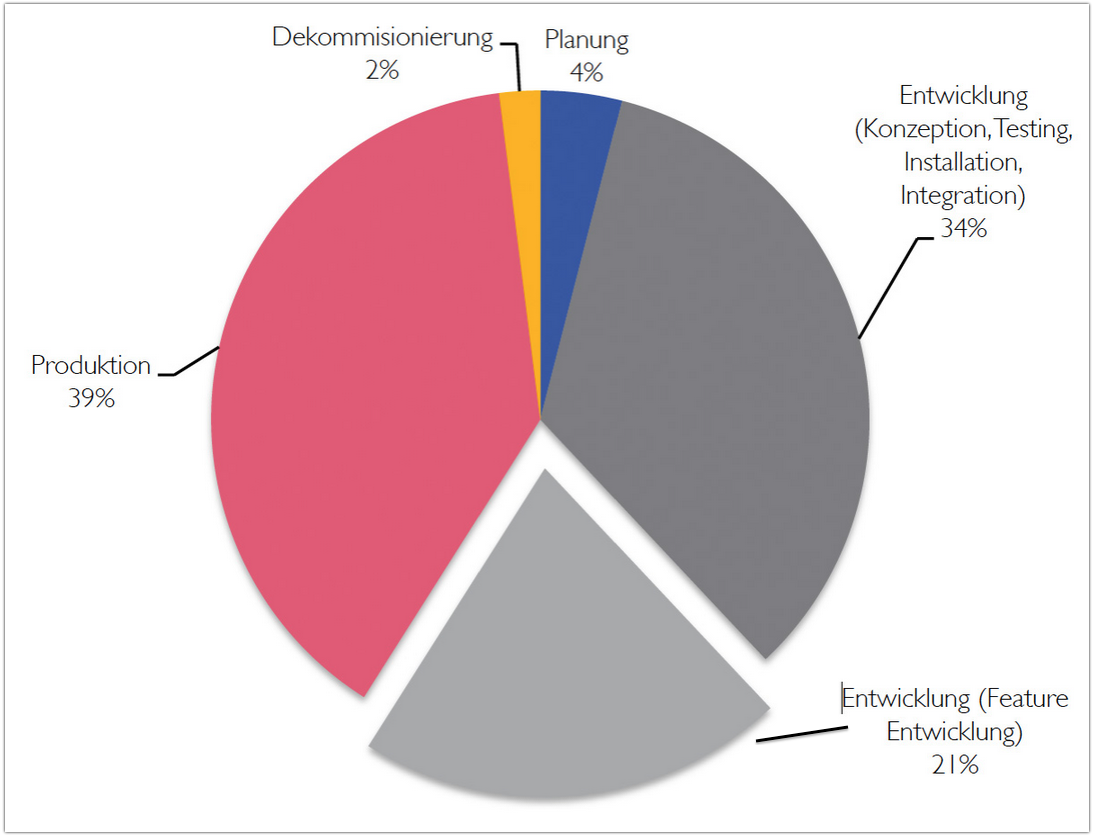
\includegraphics[width=0.9\textwidth]{img/budget_nachher.png}
	\caption[Budgetverteilung einer Applikation mit DevOps, aus \cite{siprell2014}]{Verteilung des Budgets einer Applikation auf die unterschiedlichen Bereiche mit DevOps, während ihres gesamten Lebenszyklus, aus \cite{siprell2014}}
	\label{fig:grundprinzip:budget_nachher}
\end{figure}  

Führt man das eingesparte Budget der Entwicklung zu, so kommt man nun auf einen Anteil von etwa 21\%. Dies entspricht einer Steigerung von mehr als 100\%. Das hat zur Folge, dass mit demselben Budget mehr als doppelt so viele Weiterentwicklungen einer Applikation möglich sind. Somit kann unter anderem die Kundenzufriedenheit und der Wert der Applikation erheblich gesteigert werden.

In den nachfolgenden Abschnitten wird nun beschrieben, wie die Steigerung der Effizienz erreicht werden kann. Dabei wird einzeln auf die wichtigsten Bereiche eingegangen, die DevOps umfasst und Konzepte beschrieben, wie die Probleme aus Abschnitt \ref{sec:probleme} bewältigt werden können.

\subsection{Automation von Aufgaben}
\label{sec:automation:aufgaben}
Wie in den Abschnitten \ref{sec:problem:manuellesdeployment} und  \ref{sec:releasezyklen} beschrieben, birgt die manuelle Ausführung von Aufgaben ein hohes Risiko und kann in größeren Maßstäben nicht effizient durchgeführt werden. Daher ist die oberste Priorität auf technischer Seite, die Automatisierung von Aufgaben, die bisher manuell durchgeführt wurden. Aus diesem Grund muss der komplette Prozess, von der Änderung der Software bis zum Betrieb der neuen Version, betrachtet werden \cite{wolff2014}. Reduziert man den Prozess auf ein Minimum, so umfasst er zumindest zwei Aufgaben: das Bauen der Software und das Deployment in Produktion. Ohne diese beiden Tätigkeiten würde eine Software nicht die produktive Umgebung erreichen und somit nicht für den Kunden verfügbar sein.

Im ersten Schritt kann der Build-Prozess der Software automatisiert werden. Dies ist ebenso Voraussetzung für Continuous Integration (CI) und hat sich in den letzten Jahren bereits in vielen Unternehmen etabliert. Speziell für diese Aufgabe gibt es einige Systeme am Markt wie Gradle\footnote{\url{https://gradle.org/docs/current/userguide/userguide}, Build Managament System} oder Maven\footnote{\url{https://maven.apache.org/}, Build Managament System}, die unter anderem das Abhängigkeitsmanagement erleichtern. Mit ihnen wird der Build-Prozess formalisiert und textuell erfasst. Jede Änderung an diesem Prozess kann in einem Versionsverwaltungssystem (VCS) erfasst werden. Zusätzlich dazu wird noch ein CI-Server benötigt, der den Build-Prozess ausführt und die Ergebnisse verwaltet. Ein verbreitetes Beispiel hierfür ist die freie Software Jenkins\footnote{\url{https://wiki.jenkins-ci.org/display/JENKINS/Meet+Jenkins}, erweiterbarer CI/CD-Server}. Somit kann jede Änderung am Source Code sofort und reproduzierbar gebaut werden. Jedes Software Artefakt kann ohne manuellen Aufwand genau reproduziert werden.

Als nächstes muss das Deployment des Software Artefaktes automatisiert werden. Hierfür ist es nötig, ein sogenanntes Konfigurationsmanagement-System einzuführen. In diesem System wird der Prozess des Deployments formalisiert und textuell erfasst. Der Prozess wird dadurch jederzeit reproduzierbar. Bei der Umsetzung muss unbedingt beachtet werden, dass das Deployment idempotent gestaltet wird. Das bedeutet, dass kein bestimmter Zustand angenommen werden darf. Nur der Endzustand ist relevant. Ein wiederholtes Ausführen des Prozesses muss als Ergebnis immer den gewünschten Endzustand haben. Damit wird erreicht, dass der Prozess jederzeit ausgeführt werden kann. Es ist kein Vorwissen über den Zustand des Zielsystems nötig und ein Deployment kann deswegen jederzeit durchgeführt werden.

\begin{figure}[ht]
	\centering
	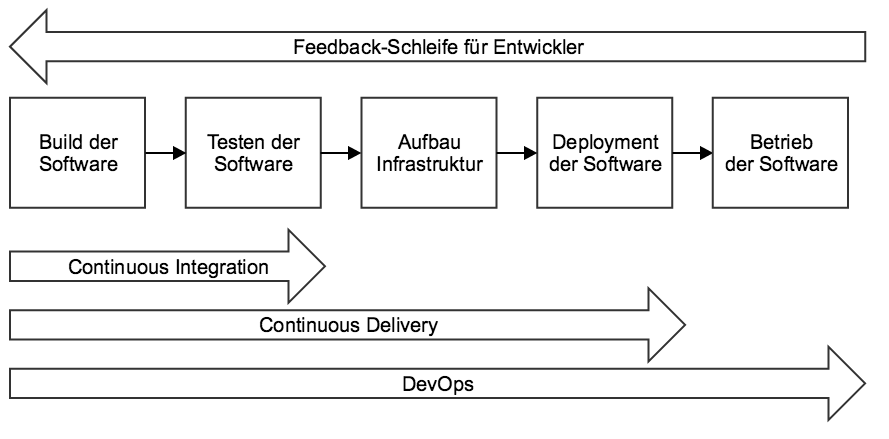
\includegraphics[width=0.95\textwidth]{img/auto_aufgaben.png}
	\caption[Grundlegende zu automatisierende Aufgaben]{Grundsätzliche Aufgaben die im Software Releasezyklus automatisiert werden müssen, um die Effizienz zu steigern.}
	\label{fig:devops:automation_aufgaben}
\end{figure} 

Beispiele für solche Konfigurationsmanagement-Systeme sind Ansible\footnote{\url{http://docs.ansible.com/}}, Puppet\footnote{\url{https://puppetlabs.com/puppet/what-is-puppet}} oder Chef\footnote{\url{https://docs.chef.io/}}. Sie bieten bereits viele Konzepte, um die Entwicklung von idempotenten Prozessen zu erleichtern. Wie auch beim Build-Prozess wird ein System benötigt, das diese Prozesse ausführt und die Ergebnisse verwaltet. Ansonsten wäre zwar der Prozess selbst automatisiert, aber man könnte nicht reproduzieren wer den Prozess wann ausgeführt hat. Die Nachvollziehbarkeit geht verloren. Für diese Aufgabe kann ebenfalls Jenkins verwendet werden, da dieser durch Plugins von einem CI-Server zu einen Continuous Deployment Server erweitert werden kann.

Dies sind aber nur die zwei grundlegenden Aufgaben, die in jedem Fall automatisiert werden müssen \cite{humble2010, wolff2014}. Es gibt noch viele weitere Aufgaben, die beachtet werden müssen. \autoref{fig:devops:automation_aufgaben} zeigt typische Aufgaben, die in vielen Prozessen eines Software-Releasezyklus vorkommen. So muss auch die Infrastruktur für die Software automatisiert bereitgestellt (Abschnitt \ref{sec:devops:infrastructureascode}) oder das Testen der Software effizienter gestaltet werden (Abschnitt \ref{sec:automation:tests}). Die Zusammenführung aller automatisierten Aufgaben in einen reproduzierbaren Prozess wird oft als Delivery Pipeline bezeichnet. Auf diese Pipeline wird in Abschnitt \ref{sec:devops:pipeline} noch genauer eingegangen.

\subsection{Automatisiertes Testen}
\label{sec:automation:tests}
Der meiste Aufwand beim Testen eines neuen Releases fällt für Regressionstests an. Je umfangreicher die Applikation, desto mehr Aufwand ist hier pro Release nötig. Das Testen von neuen Funktionen beträgt oft nur einen Bruchteil des Testaufwands. Durch DevOps und Continuous Delivery werden die Releasezyklen verkürzt und die in Abschnitt \ref{sec:releasezyklen} beschriebenen Probleme gelöst. Allerdings hat das zur Folge, dass häufiger getestet werden muss. Hierbei ist manuelles Testen, im besonderen für Regressionstest, nicht mehr effizient genug und hat hohe Kosten zur Folge. 
Außerdem haben manuelle Tests den gravierenden Nachteil, dass sie nicht eindeutig nachvollziehbar sind. Die durchgeführten Schritte können bei der Fehlersuche nicht mehr genau reproduziert werden. Aus diesen Gründen müssen auch die Tests automatisiert werden, um sie schneller und öfter durchführen zu können und gleichzeitig den Aufwand zu reduzieren \cite{wolff2014}.

Bei DevOps und Continuous Delivery werden bei jeder Änderung der Software die Tests durchgeführt. Das ermöglicht, dass der Entwickler sofort Feedback bekommt, ob seine Änderung einen Fehler verursacht. Ist dies der Fall, kann durch die geringe Menge an Änderungen die Fehlerquelle leicht identifiziert werden. Um eine gute Aussagekraft der Tests zu erreichen, müssen sie möglichst alle Bereiche der Applikation abdecken. Laut \cite{wolff2014} sind folgende Typen von Tests maßgeblich zu beachten:

\begin{itemize}
	\item \textbf{Unit Tests:} Sie sind die einfachsten und schnellsten Tests und stellen die grundlegende Funktionalität von Modulen sicher. Mit ihnen wird die interne Implementierung von Modulen überprüft, womit sie zu den White-Box-Tests gehören. Sie prüfen allerdings immer nur ein Modul und nicht das Zusammenspiel mehrerer Module. Dies muss durch Systemtests abgedeckt werden. Ein Beispiel für eine Technologie für den Einsatz von Unit Tests ist JUnit.\footnote{\url{http://junit.org/}, Unit Test Framework für Java Applikationen}
	\item \textbf{Systemtests:} Sie prüfen ein System als Ganzes und somit das Zusammenspiel mehrerer Komponenten. Hier können auch externe Systeme miteinbezogen werden. Da die interne Implementierung irrelevant ist, zählen Systemtests meist zu den Black-Box-Tests. Sie sind eine der wichtigsten Testtypen, da mit ihnen die korrekte Funktionsweise einer Applikation überprüft wird.
\end{itemize}

Beiden Typen von Tests können laut \cite{wolff2014} auf folgende Arten durchgeführt werden. Diese Arten stehen orthogonal zu den Testtypen und ermöglichen kombiniert, in den meisten Fällen, eine gute Testabdeckung einer Applikation.
	
\begin{itemize}
	\item \textbf{Funktionale Tests:} Sie testen die Applikation auf funktionale Anforderungen und somit auf die Erfüllung bestimmter Anwendungsfälle. Funktionale Tests fungieren oft als Akzeptanztests. Akzeptanztests sind vor allem für die Anwender von Relevanz. Sofern sie zusammen mit den Anwendern definiert und akzeptiert wurden, können sie auch als Abnahmekriterium für die Applikation dienen. Sind die Akzeptanztests erfüllt, so hat die Applikation eine ausreichend hohe Qualität für den Einsatz.
	
Die Durchführung kann über spezielle APIs oder die Benutzeroberfläche (GUI) erfolgen. Tests über die GUI sind allerdings fragiler, als Tests über eine definierte API. Sie können bereits durch einfache Designänderungen der Oberfläche gebrochen werden, obwohl kein Fehler vorliegt. Für GUI Tests kann beispielsweise Selenium\footnote{\url{http://www.seleniumhq.org/}, Testing Framework zur Simulation von Benutzerinteraktionen} und für API Tests SoapUI\footnote{\url{http://www.soapui.org/about-soapui/what-is-soapui.html}, Testing Framework für APIs} verwendet werden.
	
	\item \textbf{Nicht-Funktionale Tests:} Diese kontrollieren die Applikation auf bestimmte Qualitätskriterien. Kapazitätstests überprüfen beispielsweise die Performanz einer Applikation. Sie gestalten sich allerdings schwierig, da Applikationen meist nicht linear auf Last reagieren. Daher werden Testreihen durchgeführt, um festzustellen, ab welcher Last die Performanz einbricht. Die getestete Umgebung muss für aussagekräftige Resultate sehr ähnlich der produktiven Umgebung sein. Das ist aus wirtschaftlichen Gründen oft nicht möglich. Daher sollte zusätzlich ein entsprechendes Monitoring installiert werden, das die aktuelle Performanz des Systems misst und potentielle Performanzprobleme großteils voraussagt. So bleibt ausreichender Handlungsspielraum um darauf reagieren zu können. Für Kapazitätstests können unter anderem FunkLoad\footnote{\url{http://funkload.nuxeo.org/intro.html}, Framework für Funktionale und Performanztests} oder Gatling\footnote{\url{http://gatling.io/docs/2.1.6/}, Framework spezialisiert auf Performanztests} verwendet werden.
	\item \textbf{Explorative Tests:} Die bisher genannten Arten von Tests sind vor allem für Regressionstests gebräuchlich. Explorative Tests beschäftigen sich hingegen mit neuen Funktionalitäten und nicht quantitativ messbaren Aspekten, wie die Verwendbarkeit der Applikation. Diese Art von Test lässt sich allerdings nur schwer automatisieren. Daher können sie in vielen Fällen nur manuell durchgeführt werden. Da sich der zeitliche Aufwand für automatisierte Regressionstests auf ein Minimum begrenzt, steht für exploratives testen ausreichend Zeit zur Verfügung. Neue Funktionen erfordern allerdings nach geraumer Zeit die Überführung explorativer in automatisierte Tests. 
\end{itemize}

Eine von \cite{wolff2014} empfohlene Verteilung und Gewichtung der unterschiedlichen Arten von Tests für viele Anwendungsfälle ist in \autoref{fig:testpyramide} dargestellt.

\begin{figure}[ht]
	\centering
	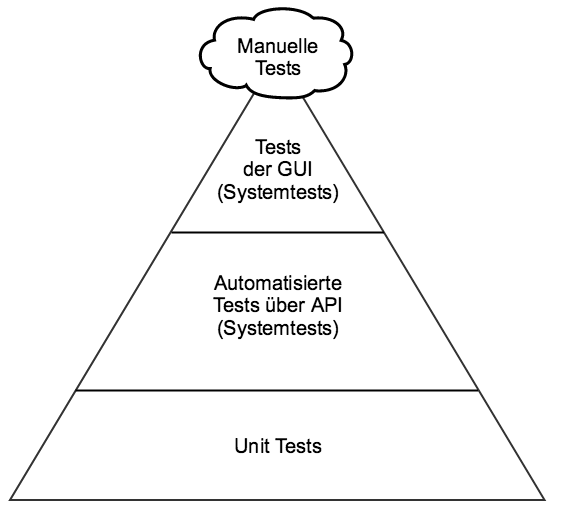
\includegraphics[width=0.65\textwidth]{img/testpyramide.png}
	\caption[Testpyramide, adaptiert aus \cite{wolff2014}]{Empfohlene Verteilung der Tests für viele Applikationen, visualisiert Anhand der Testpyramide, adaptiert aus \cite{wolff2014}}
	\label{fig:testpyramide}
\end{figure}  

Die meisten Tests sollten über Unit-Tests erfolgen. Sie bilden die Basis für eine funktionierende Applikation. Darauf aufbauend sollte es eine große Menge an funktionalen und nicht-funktionalen Tests geben. Für eine höhere Stabilität der Tests sollten diese eine API der Applikation nutzen. Zusätzlich kann es noch Tests über die GUI geben, um diese mittels automatisierten Tests zu überprüfen. Ansonsten kann das Backend der Applikation fehlerfrei sein, die dazugehörige GUI aber nicht korrekt funktionieren. Den kleinsten Anteil bilden manuelle Tests, zur explorativen Überprüfung der Applikation. Sie sollten in sehr eingeschränktem Ausmaß nötig sein.

Die automatisierten Tests decken den Bereich der Regressionstests ab und testen vor allem bestehende Funktionalitäten. Da sie meist den Großteil des Testaufwands ausmachen, steckt hier viel Optimierungspotential. Ein Sonderfall, bei dem manuelles Testen nötig ist, sind neue Funktionalitäten. Dies kann allerdings bereits in der Entwicklung berücksichtigt werden, indem Test Driven Development\footnote{\url{http://www.infoq.com/presentations/tdd-original}, Einstündige Einführung in TDD} betrieben wird. Dabei werden zuerst die Tests geschrieben und die Implementierung ist erst abgeschlossen, wenn die Tests fehlerlos ausgeführt werden. Dies setzt aber voraus, dass die Abnahmekriterien bereits vor der Entwicklung feststehen.

Automatisierte Tests müssen allerdings nicht allumfassend sein. Jeden Grenzfall zu testen würde zuviel Aufwand in Anspruch nehmen, manuell wie auch automatisiert. Daher sollten die Tests die Grundfunktionalitäten der Applikation sicherstellen. Sofern alle Tests erfolgreich ausgeführt werden, sollte die Applikation eine ausreichend hohe Qualität für den Einsatz in Produktion besitzen. Fehler können nie vollständig ausgeschlossen werden, aber durch DevOps und Continuous Delivery ist die Möglichkeit gegeben, schnell auf sie reagieren zu können. Für Software-Bereiche mit besonders hohen Qualitätsanforderungen, wie beispielsweise Medizintechnik-Software, könnte dieser Ansatz nicht ausreichend passabel sein. Hierbei empfiehlt es sich, das Deployment bis zur Testumgebung zu automatisieren. Das Deployment auf die produktive Umgebung kann per manuellen Trigger durchgeführt werden. Automatisierte Tests können aber auch hier den Aufwand des Testens erheblich verringern.

\subsection{Infrastruktur Management (Infrastructure as Code)}
\label{sec:devops:infrastructureascode}
Bei der Bereitstellung der grundlegenden Infrastruktur für den Betrieb einer Applikation können manuelle Fehler passieren (siehe Abschnitt \ref{sec:probleme:infrastruktur}). Das betrifft nicht nur das Betriebssystem einer Maschine, sondern auch etwaige Drittsysteme, die für eine Applikation benötigt werden. Diese Probleme werden gelöst bzw. verringert, wenn die Infrastruktur automatisiert erstellt wird. Das in Abschnitt \ref{sec:automation:aufgaben} beschriebene Konfigurationsmanagementsystem  kann dafür eingesetzt werden.

Die Erstellung einer Infrastruktur oder die Installation eines Drittsystems kann als Deployment einer Software angesehen werden \cite{wolff2014}. In Zeiten der Virtualisierung ist die Zielmaschine nur mehr Software und kann automatisiert deployed werden. Es müssen also Prozesse im Konfigurationsmanagement-System geschaffen werden, um die Erstellung der virtuellen Maschine, inklusive Installation des Betriebssystems und etwaiger Drittsysteme, zu übernehmen. So ist sichergestellt, dass dieser Zustand der Infrastruktur jederzeit wiederhergestellt werden kann. Bei einem Cluster wird außerdem jede Maschine gleich erstellt. Eine unterschiedliche Konfiguration einzelner Maschinen ist nicht mehr möglich. Zusätzlich hat man die Möglichkeit, komplette Umgebungen ohne manuellen Aufwand und mit geringen Kosten zu erstellen. So können für einzelne komplexe Testszenarien spezielle Umgebungen aufgebaut oder Zero-Downtime-Release (Abschnitt \ref{sec:devops:pipeline}) durchgeführt werden.

Ein wichtiger Aspekt hierbei ist, dass Personen keine Änderungen mehr manuell auf Maschinen durchführen dürfen. Jede Änderung einer Konfiguration des Betriebssystems, einer Drittsoftware oder ähnlichem darf nur mehr über den automatisierten Prozess erfolgen. Ansonsten können sich Konfigurationen unterscheiden bzw. kann eine Änderung nach erneutem Deployment wieder verschwunden sein. Wenn das Konfigurationsmanagementsystem in einem VCS eingecheckt ist, hat man den Vorteil, dass jede Änderung anhand der Historie ersichtlich ist. Man kann nachvollziehen wer welche Änderung wann durchgeführt hat, im Gegensatz zu den manuellen Tätigkeiten. Daher die Bezeichnung Infrastructure-as-Code, da die Infrastruktur wie Source Code behandelt wird \cite{wolff2014}.

Ähnlich wie in Abschnitt \ref{sec:automation:aufgaben} muss auch das Deployment der Infrastruktur idempotent gestaltet werden, damit der Prozess jederzeit ausführbar ist. Bei einer kompletten Infrastruktur müssen wesentlich mehr Bereiche beachtet werden, als beim Deployment einer einzelnen Applikation. Bei einer Applikation sind oft nur wenige Teile und Konfigurationen betroffen, die im Konfigurationsmanagementsystem verwaltet werden. Bei einer Infrastruktur ist die Zahl der Konfigurationen, die verändert werden können, wesentlich höher. Alle Konfigurationen im Prozess zu beachten, würde diesen unnötig verkomplizieren. Um dies zu lösen, hat \cite{fowler2012} im Jahr 2012 den sogenannten Phoenix Server beschrieben. Dies bezeichnet einen Server, der jederzeit abgerissen und neu aufgebaut werden kann, um wieder einen genau definierten Zustand zu erreichen. Somit werden auseinander laufende Konfigurationen verhindert. Darauf aufbauend beschrieb \cite{morris2013} den Immutable\footnote{deutsch: unveränderbar} Server. Ein Server der nach initialer Erstellung nicht mehr verändert werden darf. Sind Änderungen notwendig, so muss der aktuelle Server durch einen Neuen, mit aktualisierter Konfiguration, ersetzt werden. Bei diesem Ansatz werden nachträgliche Fehlkonfigurationen vermieden. Ein weiterer Vorteil ist, dass der Prozess zum Erstellen der Infrastruktur regelmäßig getestet und so zur Routinearbeit wird. 

Neben der Bereitstellung der Infrastruktur müssen weitere infrastrukturelle Aufgaben betrachtet werden. Für die Installation des Betriebssystems muss dieses in Form eines Image bereitgestellt werden. Dieses muss genau definiert sein und soll wiederum automatisiert erstellt werden. Darüber hinaus ist es von Vorteil, sich selbst verwaltende Applikationen zu verwenden, um manuelle Arbeit zu vermeiden. Eine Applikation, die beispielsweise oft neu konfiguriert wird, ist der Loadbalancer. Jedes mal wenn eine neue Maschine erstellt bzw. eine gelöscht wird, muss die Konfiguration des Loadbalancers entsprechend angepasst werden. Deshalb sollte die Konfiguration des Loadbalancer automatisch erzeugt werden. Dafür ist eine sogenannte Service Registry notwendig, in der alle vorhandenen Maschinen verzeichnet sind. Diese kann beispielsweise mit Hilfe von Consul\footnote{\url{https://www.consul.io/intro/}, verteilte Service Registry von Hashicorp} aufgebaut werden. Aus der Service Registry können anschließend Konfigurationen vielfältig erzeugt werden. 

\subsection{Die Deployment Pipeline}
\label{sec:devops:pipeline}
Die einzelnen Phasen einer Software, von der Fertigstellung der Entwicklung bis zum Deployment in der produktiven Umgebung, werden in einer sogenannten Deployment Pipeline zusammengefasst \cite{humble2010}. Eine Applikation muss die Deployment Pipeline vollständig durchlaufen, bis sie produktiv eingesetzt wird. Die Pipeline kann je nach Unternehmen und Applikation im Detail unterschiedlich aufgebaut sein. Allerdings lässt sich jede Pipeline auf das in \autoref{fig:deployment_pipeline} gezeigte grundsätzliche Schema reduzieren.

\begin{figure}[ht]
	\centering
	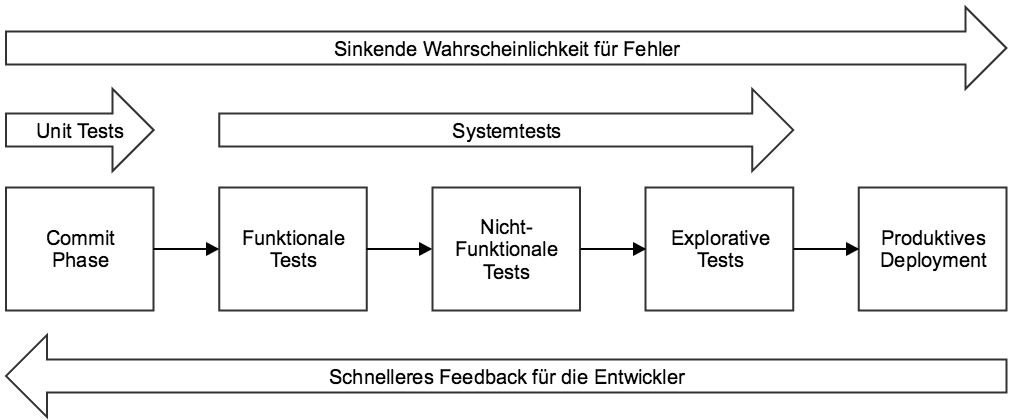
\includegraphics[width=0.99\textwidth]{img/deployment_pipeline.png}
	\caption[Schema einer Deployment Pipeline, adaptiert aus \cite{humble2010} und \cite{wolff2014}]{Grundsätzliches Schema einer Deployment Pipeline. Jede abgeschlossene Phase steigert die Produktionsreife der Applikation. Adaptiert aus \cite{humble2010} und \cite{wolff2014}.}
	\label{fig:deployment_pipeline}
\end{figure} 

Durch diesen Aufbau garantiert die Pipeline, dass die Entwickler so schnell wie möglich Feedback zu gemachten Änderungen bekommen. Fehler werden frühestmöglich erkannt und können daher leichter und kosteneffizienter behoben werden. Die einzelnen Phasen erfüllen laut \cite{humble2010} und \cite{wolff2014} folgende Aufgaben:

\begin{itemize}
	\item \textbf{Commit Phase:} Diese Phase ist der Start der Deployment Pipeline und wird getriggert, sobald die Entwickler eine Änderung in das VCS einchecken. Jeder Commit löst eine neue Instanz der Pipeline aus. Zuallererst wird die Applikation gebaut und ein Artefakt erzeugt. Sobald dies abgeschlossen ist, werden die Unit-Tests ausgeführt. Nur wenn alle diese Prozesse erfolgreich durchgeführt sind, darf die Commit Phase abgeschlossen werden. Das Ergebnis ist ein Software Artefakt, das ein Mindestmaß an Qualität aufweist und keine groben Fehler enthält. Üblicherweise steht das Ergebnis der Commit Phase nach wenigen Minuten fest. Die Entwickler bekommen hierbei schnellstmöglich Feedback.
	\item \textbf{Funktionale Tests:} Anschließend wird das Artefakt in einer möglichst produktionsähnlichen Umgebung deployed und funktionale Systemtests durchgeführt. Sofern dies weitgehend automatisiert ist, kann für jede Instanz der Pipeline eine eigene Testumgebung aufgebaut werden. Sind die Systemtests erfolgreich, so erfüllt das Artefakt jedenfalls die technischen und funktionalen Anforderungen und weist somit bereits eine hohe Qualität auf. Üblicherweise sollte das Ergebnis dieser Phase in weniger als einer Stunde feststehen. Die Entwickler können sich dann weitgehend sicher sein, dass ihre Arbeit eine ausreichende Qualität aufweist. Im Gegensatz dazu erfordert dies bei klassischen Prozessen meist einige Tage bis Wochen.
	\item \textbf{Nicht-Funktionale Tests:} Nachdem die funktionale Qualität sichergestellt ist, sollten auch nicht-funktionale Systemtests durchgeführt werden. Üblicherweise sind dies Performanz- und Kapazitätstests. Diese garantieren beispielsweise, dass durch eine Änderung, die Performanz nicht drastisch beeinträchtigt wurde. Nach Abschluss dieser Phase hat das Artefakt meist eine ausreichend hohe Qualität für ein Deployment in der produktiven Umgebung. Die Wahrscheinlichkeit für einen Fehler ist bereits auf ein Minimum reduziert. Das Ergebnis dieser Phase sollte üblicherweise nach einem Tag zur Verfügung stehen.
	\item \textbf{Explorative Tests:} Diese Phase kann als optional angesehen werden, allerdings ist sie Bestandteil vieler Pipelines. Hier wird das Artefakt manuell getestet, um beispielsweise neue Funktionalitäten zu überprüfen. Bis hierher wurde die Pipeline vollständig automatisch durchlaufen. Diese Phase muss jedoch manuell bestätigt werden um sie erfolgreich abzuschließen. Sind hingegen keine explorativen Tests notwendig, kann die Pipeline bis zum Deployment auf Produktion vollständig automatisch durchlaufen werden.
	\item \textbf{Produktives Deployment:} In der letzten Phase wird das getestete und mittlerweile qualitativ hochwertige Artefakt in der produktiven Umgebung deployed. Oftmals ist der Beginn dieser Phase eine manuelle Bestätigung und nicht der erfolgreiche Abschluss der vorangegangenen Phase. Insbesondere dann, wenn die Pipeline eine Phase für exploratives Testen erfordert. Ist die Pipeline hingegen vollständig automatisiert, sind selbst vielzählige Deployments pro Tag realistisch\footnote{\url{http://www.infoq.com/presentations/Continuous-Deployment-50-Times-a-Day}}.
\end{itemize}

Wenn eine der oben genannten Phasen nicht erfolgreich abgeschlossen wird, muss die Deployment Pipeline abgebrochen werden, da es keinen Sinn macht, weitere Phasen zu durchlaufen. Bei Abbruch müssen die zuständigen Entwickler entsprechend benachrichtigt werden, um auf das negative Ergebnis zu reagieren. Je weiter die Pipeline zum Zeitpunkt des Abbruchs durchlaufen wurde, desto länger mussten die Entwickler auf Feedback warten. Allerdings sinkt mit jeder abgeschlossenen Phase die Wahrscheinlichkeit für Fehler. Daher können die Entwickler bereits eine Stunde nach erfolgtem Commit, mit hoher Wahrscheinlichkeit davon ausgehen, keine Fehler verursacht zu haben. Der Fokus kann also auf die nächste Aufgabe gelegt werden.

Eine Grundbedingung einer Deployment Pipeline ist, dass das gebaute Artefakt aus der Commit Phase in jeder weiteren Phase verwendet wird. Das Artefakt darf pro Instanz der Pipeline nur ein einziges mal gebaut werden. Es darf also nicht für jede Phase ein eigenes Artefakt gebaut werden. In diesem Fall könnte durch den erneuten Buildprozess ein Fehler entstehen, der durch die Tests der Commit Phase aufgefallen wäre, später aber nicht mehr entdeckt wird. Im schlimmsten Fall wird dieser Fehler dann in Produktion deployed. 

Durch die Verwendung einer Deployment Pipeline ergeben sich zusammenfassend folgende Vorteile:
\begin{itemize}
	\item Die Feedback-Zyklen für die Entwickler reduzieren sich auf ein Minimum. Fehler können schneller gefunden und mit weniger Kosten behoben werden.
	\item Die Deployment-Prozesse werden laufend getestet, da bei der Transition zwischen den Phasen ein Deployment auf Testumgebungen erfolgt. Dadurch erhöht sich dessen Sicherheit und das Fehlerrisiko sinkt.
	\item Die Qualität der Software wird durch die vielen Testphasen zu einer hohen Wahrscheinlichkeit sichergestellt.
\end{itemize}

\paragraph{Deployment Möglichkeiten:} 
Kritischste Phase der Pipeline ist das Deployment in die produktive Umgebung. Obwohl der Erfolg eines Deployments durch Automatisierung nahezu sichergestellt wird, können Fehler nie vollständig ausgeschlossen werden. Um das Risiko zu minimieren, gibt es mehrere Möglichkeiten, wie ein Deployment durchgeführt werden kann. Laut \cite{humble2010} werden folgende drei Vorgehensweisen am häufigsten eingesetzt:

\begin{itemize}
	\item \textbf{Rollout:} Dies ist die einfachste Variante für ein Deployment. Hierbei wird das gesamte System mit einer neuen Version aktualisiert. Dies geschieht meist während eines Wartungsfensters, bei dem die Applikation nicht erreichbar ist. Nach dem Rollout ist ausschließlich die neue Version für die Benutzer aktiv. Gibt es Fehler nach dem Deployment kann ein Rollback durchgeführt werden. Dies hat aber wiederum einen Ausfall der Applikation zur Folge.
	\item \textbf{Blue/Green Deployment:} Hierbei wird die neue Version auf einer komplett getrennten Umgebung deployed. Ist das Deployment abgeschlossen, wird auf diese Umgebung umgeschaltet. Ab diesem Zeitpunkt verwenden alle Benutzer die neue Version. Es entsteht also keine Ausfallzeit (Zero-Downtime-Release). Diese Methode bedingt einen hohen Ressourcenverbrauch, da zwei produktive Umgebungen betrieben werden müssen. Wird außerdem eine Datenbank verwendet, so müssen die Datenbanken der beiden Umgebungen synchron gehalten werden. 
	\item \textbf{Canary Release:} Bei dieser Vorgehensweise wird die neue Version auf wenige Maschinen im Cluster deployed. Sie wird dadurch nur von einem Bruchteil der Benutzer verwendet und so in Produktion getestet. Ein Rollback ist sehr einfach durchzuführen, indem die aktualisierten Maschinen wieder entfernt werden. Funktioniert die Version, so kann sie ohne Ausfallzeit sukzessive auf alle Maschinen ausgerollt werden. Diese Vorgehensweise ist jedoch für viele Arten von Applikationen nicht praktikabel, wenn beispielsweise die neue Versionen ein angepasstes Datenbankschema benötigt.
\end{itemize}

Abgesehen vom klassischen Rollout kann mit Blue/Green Deployments bzw. Canary Releases neben der Risikominimierung auch ein Rollback vereinfacht werden. Allerdings haben diese beiden einen wesentlich höheren Ressourcenverbrauch als der klassische Rollout.

\subsection{Unternehmenskultureller Aspekt von DevOps}
\label{sec:devops:firmenkultur}
In Abschnitt \ref{sec:problem:kluft} wurden Probleme beschrieben, die durch die strikte Trennung von Entwicklung und Betrieb entstehen. Die Konzepte von DevOps beschäftigen sich neben den technologischen Aspekten auch mit diesen Problemen. Laut \cite{walls2013} ist es für den Erfolg von DevOps essentiell, die Zusammenarbeit zwischen Entwicklung und Betrieb zu verbessern. Ein großes Hindernis bei der Zusammenarbeit sind die unterschiedlichen Ziele und Werte der Teams. Sie müssen für eine erfolgreiche Zusammenarbeit einheitlich definiert werden. Hierbei muss ein Kompromiss zwischen Stabilität und flexibler Entwicklung gefunden werden, bei dem der Schwerpunkt entsprechend den Anforderungen des Unternehmens individuell definiert werden kann. Dabei sollte laut \cite{wolff2014} für beide Teams der Service immer im Vordergrund stehen, um diesen bestmöglich an die Kunden zu liefern.

In der Literatur zu DevOps, wie beispielsweise \cite{humble2014, peschlow2012, brown2014}, wird eine verbesserte Kommunikation als Schlüsselelement angeführt. Die Barrieren zwischen Entwicklung und Betrieb müssen abgebaut und die Kommunikation verbessert werden. Bei Problemen ist gegenseitige Schuldzuweisung, die häufig Praxis ist, unter allen Umständen zu vermeiden. Für die Kunden ist es nicht relevant, wer einen Fehler verursacht hat. Deswegen müssen die Mitarbeiter einen lösungsorientierten Ansatz verfolgen. Wichtigstes Ziel ist es, den Fehler gemeinsam so schnell wie möglich zu beheben. Es ist lediglich wichtig, wie der Fehler entstanden ist und wie dieser in Zukunft vermieden werden kann. Das wird auch im serviceorientierten Ansatz von \cite{wolff2014} angeführt. 

Um eine effiziente Zusammenarbeit zu erreichen, muss neben verbesserter Kommunikation das vorhandene Wissen beider Teams ausgetauscht werden. Dies schafft Synergien, um Applikationen effizienter betreiben zu können. Einerseits sollen die Entwickler in den Betrieb mit eingebunden werden und Verantwortung für erstellte Applikationen übernehmen. Das Betriebsteam schafft die Grundlagen für die Entwickler und unterstützt sie, um ihre Applikationen selbst bestmöglich betreiben können. Andererseits sollen Entwickler das Betriebsteam bereits in der Planungsphase der Applikation mit einbeziehen. Dadurch kann der Betrieb bereits in der Entstehung wichtige Vorschläge liefern, um die Betriebstauglichkeit der Applikation zu erhöhen.
Weitere Vorteile die sich daraus ergeben sind, dass der Betrieb beim Aufbau lokaler Entwicklungsumgebungen behilflich sein kann und somit diese schon mehr an die produktive Umgebung angleichen. Die Entwicklung wird dadurch wesentlich effizienter. Außerdem hat die Entwicklung mehr Freiheiten bei der Wahl von Technologien und dem Aufbau der Infrastruktur. Sie müssen allerdings auch entsprechend die Verantwortung für deren Betrieb übernehmen. Diese Vorgehensweise setzt aber ein hohes Maß an Vertrauen und Respekt untereinander voraus. Die kulturelle Anpassung an DevOps ist deswegen ein langfristiger Prozess, der Zeit und entsprechende Führung durch Vorgesetzte benötigt. Nur wenn diese neue Unternehmenskultur von allen Ebenen unterstützt und gelebt wird, ist ein erfolgreiches Umdenken möglich \cite{walls2013}.

Betrachtet man viele Unternehmen, so sind Entwicklung und Betrieb oft getrennt. Eine Praxis die \cite{wolff2014} empfiehlt ist, diese beiden Bereiche zu vereinen und in Teams aufzuteilen. So werden kleinere Teams gebildet, die jeweils für die Entwicklung \textbf{und} den Betrieb einer Komponente\footnote{Je nach Größe des Unternehmens und der Plattform muss eine sinnvolle Trennung gefunden werden. Dieser Ansatz steht vor allem im Bezug auf die Microservice Bewegung, bei der große Monolithen in kleinere Services aufgeteilt werden. Ein Team kümmert sich vollständig um einen Microservice.} verantwortlich sind. Das jeweilige Team hat die Entscheidungskompetenz über eingesetzte Technologien und deren Betrieb. Es muss nur sicherstellen, dass die Komponente bestmöglich bereitgestellt wird. Daher ist es wichtig, die Schnittstellen zwischen den einzelnen Komponenten zu definieren und entsprechend einzuhalten. Dieser Ansatz setzt eine große Eigenverantwortung des jeweiligen Teams voraus. Man sollte besonders darauf achten, dass zwischen den Teams reger Austausch von Wissen und Zusammenarbeit herrschen. Um dies zu erreichen, ist es sinnvoll regelmäßige Wechsel von Personen zwischen den Teams zu ermöglichen bzw. zu forcieren.

Mit den technologischen Aspekten von DevOps kann bereits eine wesentliche Steigerung der Effizienz erreicht werden. Für die Lösung aller in Abschnitt \ref{sec:probleme} genannten Probleme, muss aber auch die Firmenkultur mit einbezogen werden. Nur wenn man diese beiden Komponenten entsprechend verbindet, können die Potenziale von DevOps zur Gänze genutzt werden.